\documentclass[12pt]{beamer}

\usetheme{Oxygen}
\usepackage[T1]{fontenc}
\usepackage{graphicx}
\usepackage{hyperref}
\usepackage[utf8]{inputenc}
\usepackage{thumbpdf}
\usepackage{ucs}
\usepackage{verbatim}
\usepackage{wasysym}
\usepackage{pgf,pgfarrows,pgfnodes,pgfautomata,pgfheaps,pgfshade}

\pdfinfo
{
  /Title       (Open vSwitch)
  /Creator     (Willian Paixao)
  /Author      (Willian Paixao)
}


\graphicspath{{img/}}

\title{\texttt{Open vSwitch}}
\subtitle{Um switch virtual livre}
\author{Willian Paixao \\ \href{mailto:willian@ufpa.br}{willian@ufpa.br}}
\date{\today}

\begin{document}

\frame{\titlepage}

\newcommand<>{\highlighton}[1]{%
  \alt#2{\structure{#1}}{{#1}}
}

\newcommand{\icon}[1]{\pgfimage[height=1em]{#1}}


%%%%%%%%%%%%%%%%%%%%%%%%%%%%%%%%%%%%%%%%%
%%%%%%%%%% Content starts here %%%%%%%%%%
%%%%%%%%%%%%%%%%%%%%%%%%%%%%%%%%%%%%%%%%%


\section{Introdução}

\begin{frame}
  \frametitle{Introdução}
  \framesubtitle{O que é?}
  \begin{block}{Definição}
  \begin{itemize}
    \pause
    \item Switch
    \pause
    \item Virtual
    \pause
    \item Livre
  \end{itemize}
  \end{block}
\end{frame}

\section{Funcionalidades}
\begin{frame}
  \frametitle{Funcionalidades}
  \framesubtitle{O que faz?}
  \begin{block}{Protocolos suportados}
  \begin{itemize}
    \pause
    \item Bidge
    \pause
    \item VLAN
    \pause
    \item QoS
    \pause
    \item NIC Bounding
    \pause
    \item BFD e 802.1ag
  \end{itemize}
  \end{block}
\end{frame}

\section{Exemplos}
\section{Cenário 1}
\begin{frame}
  \frametitle{Cenário 1}
  \framesubtitle{Dois hosts, quatro VMs}
  \begin{block}{Configuração da rede}
  \begin{itemize}
    \pause
    \item Duas sub redes
    \pause
    \item Dois hosts
    \pause
    \item Quatro máquinas virtuais
  \end{itemize}
  \end{block}
\end{frame}

\begin{frame}
  \frametitle{Cenário 1}
  \framesubtitle{Dois hosts, quatro VMs}
  \begin{figure}[t]
      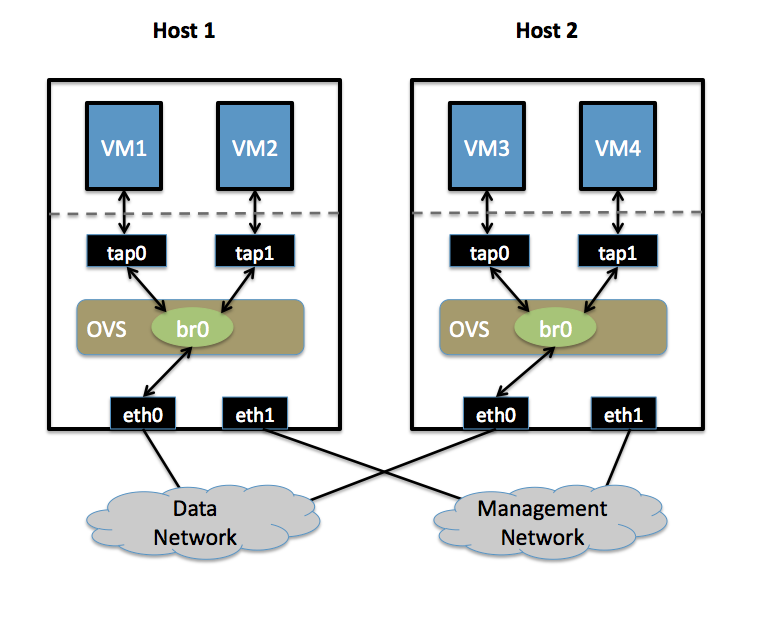
\includegraphics[width=.75\textwidth]{2host-4vm}
      \centering
  \end{figure}
\end{frame}

\section{Fancy features}
\begin{frame}
  \frametitle{Highlighting}
  \framesubtitle{Hey! Look here! here!}

  \begin{block}{A regular block}
  \begin{itemize}
    \item Normal text
    \item \highlighton{Highlighted text} to draw attention
    \item \alert{"Alert'ed" text} to spot very important information
    \item Alternatively you can
    \begin{itemize}
      \alert{\item "Alert" the item itself}
      \highlighton{\item Or "Highlight" it}
    \end{itemize}
  \end{itemize}
  \end{block}
  \begin{alertblock}{If it's very very important...}
  \alert{... you can "alert" in an "alertblock"}\\
  Ewww, nasty, heh?
  \end{alertblock}
\end{frame}

\newcommand{\putlink}[1]{%
   \pgfsetlinewidth{1.4pt}%
   \pgfsetendarrow{\pgfarrowtriangle{4pt}}%
   \pgfline{\pgfxy(1,1)}{\pgfxy(#1,1)}
}

\begin{frame}
  \frametitle{Overlay effects}
  \framesubtitle{Keep the suspense!}
  \begin{block}{Time bomb}
  \begin{enumerate}
    \item<2-> Two more to go
    \item<3-> One more to go
    \item<4-> Last chance...
    \item<5-> BOOM!
  \end{enumerate}
  \end{block}
  \begin{block}{"Animation"}<6->
    \begin{pgfpicture}{0cm}{0cm}{7cm}{2cm}
    \only<1-6>{
      \putlink{2}
    }
    \only<7>{
      \putlink{4}
    }
    \only<8>{
      \putlink{6}
    }
    \only<9>{
      \putlink{8}
    }
    \only<10>{
      \putlink{10}
    }
    \end{pgfpicture}
  \end{block}
\end{frame}

\section*{}
\frame{
  \vfill
  \centering
  \highlighton{
  \usebeamerfont*{frametitle}And now?

  \usebeamerfont*{framesubtitle}Enter the secret section
  }
  \vfill
}
\begin{frame}
  \frametitle{Contributing to this beamer style}
  \framesubtitle{We want you !}

  \begin{block}{Why?}
  \begin{itemize}
    \item Beamer is hot!
    \item This style deserves to be improved
  \end{itemize}
  \end{block}

  \begin{block}{How?}
  \begin{itemize}
    \item Grab it
    \item Improve its LaTeX code
    \item Use you artistics skills
    \item Document it
    \item Help other people to use it
    \item Use it...
  \end{itemize}
  \end{block}
\end{frame}

\begin{frame}
  \frametitle{Resources}
  \framesubtitle{If you want to improve this style}
  \begin{thebibliography}{10}

  \beamertemplatearticlebibitems

  \bibitem{beamer-homepage}
    LaTeX Beamer
    \newblock {\tt http://latex-beamer.sourceforge.net/}

  \bibitem{kdeslides}
    KDE Presentations
    \newblock {\tt http://www.kde.org/kdeslides/}

  \end{thebibliography}
\end{frame}

\frame{
  \vspace{2cm}
  {\huge Questions ?}

  \vspace{3cm}
  \begin{flushright}
    Konqi Konqueror

    \structure{\footnotesize{konqi@kde.org}}
  \end{flushright}
}

\end{document}
